\section{PDF Sicherheitsaspekte}
Etwa 40 \% der Unternehmen setzen PDFs für geschützte Inhalte ein. In den letzten 2 Jahren ist die Nutzung der elektronischen Signaturfunktion in PDFs um mehr als 150 \% gestiegen. \cite{formilo} Diese Statistik zeigt keine gute Entwicklung, da PDF-Dokumente nicht für vertrauliche Inhalte verwendet werden sollten. Obwohl PDF Verschlüsselung implementiert, erlaubt das Dateiformat eine Vielzahl von Angriffen, um die Sicherheit von PDF-Dokumenten zu untergraben. Ich werde im Folgenden die Sicherheitsmechanismen von PDF, sowie PDF Signature Spoofing und PDFex als Risikostufen für Schwachstellen näher beleuchten. \\ Neben den im weiteren Verlauf detailliert beschriebenen Attacken aus dem Jahr 2019, gibt es noch weitere Attacken auf PDF-Dokumente, die ich aber nur kurz benennen und nicht weiter ausführen werde. 2020 wurden Shadow Attacks entdeckt, die sich auf ein PDF Dokument mit 2 Inhaltsebenen beziehen. Zum einen wird Inhalt sichtbar, der beim Ersteller der Signatur angezeigt wird und zum anderen wird ein alternativer versteckter Inhalt dem Opfer gezeigt, nachdem das Dokument signiert wurde. Weitere unsichere Features würden im Jahr 2021 in PDFs untersucht. Man fand Möglichkeiten für \gls{dos} attacks, die sich auf den Host beziehen, der das Dokument bearbeitet, Information disclosure attacks, die persönliche Daten aus dem Computer des Opfers freilegen können, Data manipulation auf dem System des Opfers und Code execution auf dem Computer des Opfers. Zuletzt im Jahr 2021 wurden Sicherheitslücken in der PDF-Spezifikation entdeckt, die \gsl{eea} und \gls{ssa} realistisch machen. Nutzt der Angreifer diese Sicherheitslücken aus, so kann er den sichtbaren Inhalt eines Dokuments verändern, indem er bösartigen Inhalt über dem zertifizierten Inhalt anzeigt. Nichtsdestotrotz bleibt das Zertifikat gültig und die PDF-Anwendung zeigt keine Warnung an. \cite{pdf-insec}
\par
In den Sicherheitseinstellungen eines PDF-Dokuments können Dokumentensicherheit und Zugriffsregeln justiert werden. PDF unterstützt Verschlüsselung und die Vergabe von Passwörtern. Eventuell kann beim Öffnen einer Datei ein Passwort gefordert werden oder das Kopieren von Teilinhalten, jeglichem Inhalt, Ausfüllen von Formularfeldern, Dokumentveränderungen (z.B. Struktur, Inhalt, Kommentare), das Einbetten und Editieren von Schriften oder das Ausdrucken kann vom Ersteller des Dokuments gesperrt worden sein. Das Schwärzen von Dokumenten, d.h. ein schwarzer Balken liegt auf dem Text, führt nicht dazu, dass der geschwärzte Text aus der Datei verschwindet. Er kann weiterhin ausgelesen werden, ebenso Metadaten. 
\cite{adobe-pdf-pades}

\subsection{Digitale Signatur}
Digitale Signaturen sollen die Identität des Unterzeichners des Dokuments authentifizieren und sicherstellen, dass der Inhalt nach der digitalen Signatur nicht geändert wurde. Der Verfasser benötigt für die digitale Signatur ein Signatur-Zertifikat. Das Zertifikat bescheinigt die Echtheit der Signatur bzw. Herkunft und wird von einem möglichst vertrauenswürdigen Zertifizierungsanbieter ausgestellt. Zusätzlich können Zertifikate ablaufen oder entzogen werden und müssen gültig sein. Jede digitale Signatur kann mit einem Zeitstempel versehen werden. Ein externer \gls{zsa} belegt den Zeitpunkt, wann die digitale Signatur geleistet wurde. \cite{softx} \\
Eine digitale Signatur ist eine spezielle Art von elektronischer Signatur, die kryptographische Techniken implementiert. Im Gegensatz dazu kann eine elektronische Signatur verschiedene Formen annehmen, beispielsweise eine gescannte handschriftliche Unterschrift, ein getippter Name, eine biometrische Signatur oder eine digitale Signatur. Elektronische Signaturen sind der Oberbegriff und digitale Signaturen sind eine Unterart davon. Elektronische Signaturen bieten variierende Sicherheitsgrade. \cite{adobe-pdf-pades} \\
Digitale Signaturen verwenden asymmetrische Kryptographie. Anfangs wird ein Algorithmus zur Schlüsselgenerierung initiiert. Als Ausgabe werden ein Private Key und Public Key erzeugt. Ein Signierungsalgorithmus erstellt den einzigartigen Hash-Wert des PDF-Dokuments und verschlüsselt ihn mit dem geheimen Private Key, was die digitale Signatur als Output produziert. Zuletzt überprüft ein Signaturvalidierungsalgorithmus die Authentizität des PDF-Dokuments, indem er erneut einen Hash des Dokuments berechnet. Die Signatur wird mit dem Public Key entschlüsselt und gibt ebenfalls einen Hash aus. Falls der berechnete Hash im Signaturvalidierungsalgorithmus mit dem entschlüsselten Hash übereinstimmt, ist die Authentizität des PDF-Dokuments gesichert. \cite{signature} \\
Eine PDF-Datei ermöglicht mehrere digitale Signaturen, jedoch muss jede neue Signaturen in einem inkrementellen Update geleistet werden. Alle digitalen Signaturen muss mit einem Unterschriftsfeld im Dokument verbunden sein. Optional kann das Unterschriftsfeld mit einem Widget gekoppelt sein. Dann wird die Signatur graphisch dargestellte. Signaturen ohne Widgets sind versteckte digitale Signaturen. \cite{softx} Auf dem Markt werden Desktop-Anwendungen und Online-Validierungsservices zur Überprüfung der digitalen Signatur angeboten.



\subsection{PDF Signature Spoofing}
Die PDF-Spezifikation ist sehr ungenau im Bezug auf digitale Signaturen bzw. auf welche Art und Weise sie validiert werden müssen. PDF-Viewer haben eine hohe Toleranz beim Öffnen, Validieren und Anzeigen von beschädigten PDF-Dateien. \\
Im Jahr 2019 wurden 3 Attacken zum Vortäuschen von validen PDF Signaturen erforscht: \gls{isa}, \gls{swa} und \gls{usf}. Das attack scenario sieht wie folgt aus: Der Angreifer besitzt das signierte PDF mit einer gültigen digitalen Signatur und manipuliert es. Das manipulierte signierte PDF wird an das Opfer geschickt und die Signatur bleibt gültig, obwohl der Inhalt geändert wurde.
\\
Die \gls{isa} nutzt das incremental update Feature von PDF aus, um bösartigen Inhalt in das PDF des Opfers zu schleusen. Im Prozess des Signierens wird ein incremental update verwendet, um die Signatur zu speichern. Am Ende des Originaltrailers wird ein neuer Katalog und ein neues Signatur-Objekt als Body Updates angehängt, was den Signaturwert und Informationen über den Ersteller der Signatur enthält. Danach kommt eine updated Xref section und ein updated Trailer. Beim inremental update können Objekte mit anderem Inhalt neu definiert werden. Bei einem Spezifikation-konformem incremental update wird der updated Body hinter dem Originaltrailer am Dateiende angehängt. Darunter zeigt die updated Xref section auf das neue Objekt und der updated Trailer wird ganz am Ende angefügt. Abbildung \ref{fig:incr-update} zeigt den Vorgang des Speicherns einer digitalen Signatur mittels incremental update. \\

\begin{figure}[!htb]
	\centering
	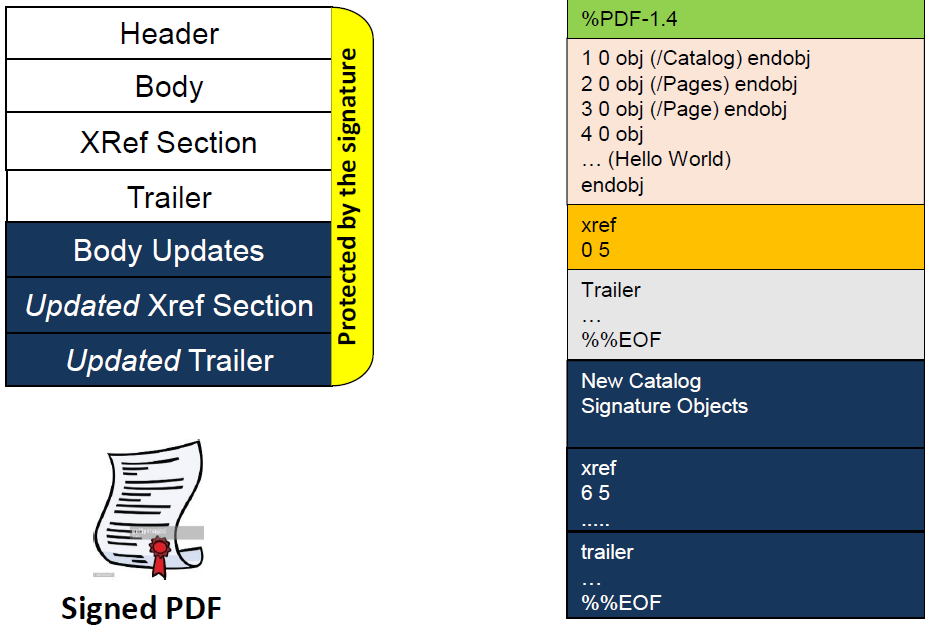
\includegraphics[width=0.8\textwidth]{"images/dig_sig_incr_up.png"}
	\caption{incremental update mit digitaler Signatur \cite{ccc-break-pdf-slides}}
	\label{fig:incr-update}
\end{figure}

Zuerst hat man bei der \gls{isa} geprüft, ob die PDF-Reader gegen eine Attacke anfällig waren, bei der hinter dem incremental update, was die digitale Signatur enthält, eine weitere Sektion mit Body Updates, Xref und Trailer angefügt wurde. Ausschließlich LibreOffice wurde mittels diese Vorgehensweise getäuscht. Alle weiteren Strategien produzieren beschädigte nicht Standard-konforme PDF-Dateien, jedoch PDF-Viewer sind sehr fehlertolerant. Als Nächstes haben die Forscher hinter dem updated Trailer des incremental updates der Signatur Body Updates hinzugefügt. Einige getestete PDF-Viewer haben lediglich überprüft, ob eine neue Xref und Trailer vorhanden sind. Da sie fehlten, blieb die Signatur gültig, die zusätzlichen Body Updates wurden ausgeführt und die Modifikation blieb ohne Warnung unbemerkt. Andere PDF-Viewer benötigten neben zusätzlichen Body Updates noch einen Trailer ohne Xref dazwischen, damit keine Warnung geworfen wurde. Die komplexeste Vorgehensweise, bei der neue Body Updates mit einer Kopie des Signatur-Objekts am Dateiende angebracht wurde, hat einige PDF-Viewer wie Foxit gezwungen die Signatur 2 Mal zu validieren und die Body Updates wurden eingefügt. In der Grafik \ref{fig:isa} werden die Techniken visualisiert, sowie die PDF-Viewer dargestellt, die anfällig für die \gls{isa}-Vorgehensweise waren.
\par

\begin{figure}[!htb]
	\centering
	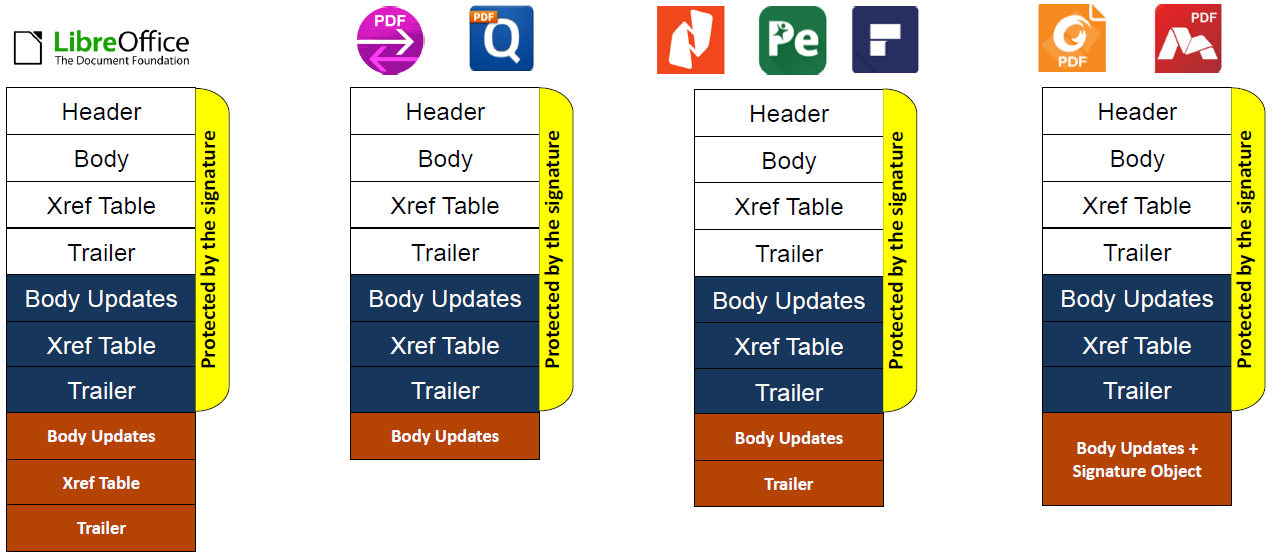
\includegraphics[width=0.8\textwidth]{"images/isa.png"}
	\caption{\gls{isa}-Methoden mit anfälligen PDF-Viewern \cite{ccc-break-pdf-slides}}
	\label{fig:isa}
\end{figure}

Bei der \gls{swa} werden die Werte der signierten /ByteRange modifiziert und Platz wird für das Einschleusen von bösartigen Inhalten geschaffen. Das Signatur-Objekt besteht aus einem /Contents entry mit dem Signaturwert und einem /ByteRange entry mit 4 Werten, was den signierten Teil im Dokument anzeigt. Die ersten 2 Einträge der /ByteRange beziehen sich auf den Beginn des Dokuments bis zum Anfang des Signaturwerts. Hingegen definieren die letzten beiden ByteRange-Einträge den Bereich nach dem Signaturwert bis zu \%\%EOF. Diese beiden Bereiche wurden nicht angerührt. Die erfolgreiche Idee war eine zweite /ByteRange hinter dem Signaturwert mit einem angepassten dritten Wert, der Platz für bösartige Objekte, etwas Padding und eine bösartige Xref, die auf die Objekte des Angreifers zeigt, zu setzen. Lediglich die Position der neuen Xref ist im Trailer vorgegeben, der nicht verändert werden kann. Das Schaubild \ref{fig:swa} zeigt, wie die \gls{swa} arbeitet.
\par

\begin{figure}[!htb]
	\centering
	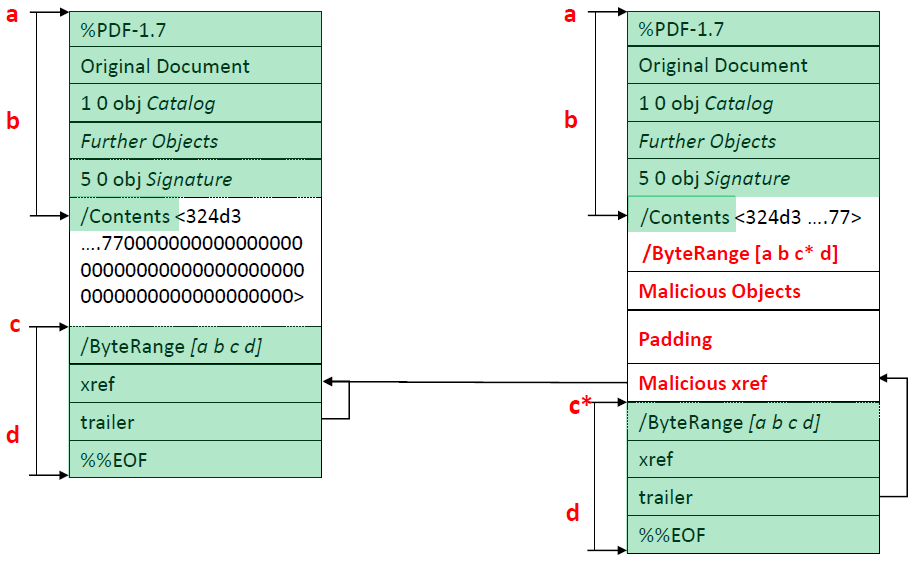
\includegraphics[width=0.8\textwidth]{"images/sig_wrap_attack.png"}
	\caption{\gls{swa}-Methodik \cite{ccc-break-pdf-slides}}
	\label{fig:swa}
\end{figure}

Mittels \gls{usf} wird die Signaturvalidierung außer Kraft gesetzt. Dennoch wird die Meldung „PDF is validly signed" dem Benutzer angezeigt. Vor allem die Adobe-Produkte waren anfällig für diese Attacke. Die Vorgehensweise gestaltete sich wie folgt: Die Forscher versuchten /Contents oder /ByteRange der Signatur entweder wegzulassen oder unüblichen Werten wie kein Wert oder null zuzuweisen. Zwei PDF-Viewer versagten, wenn man /Contents auf 0 Bytes setzte. Das Weglassen der /ByteRange oder das Gleichsetzen mit null brach die Sicherheitsmechanismen von Adobe. Die Grafik \ref{fig:usf} zeigt die \gls{usf}-Varianten, die von den Forschern getestet wurde.
\par

\begin{figure}[!htb]
	\centering
	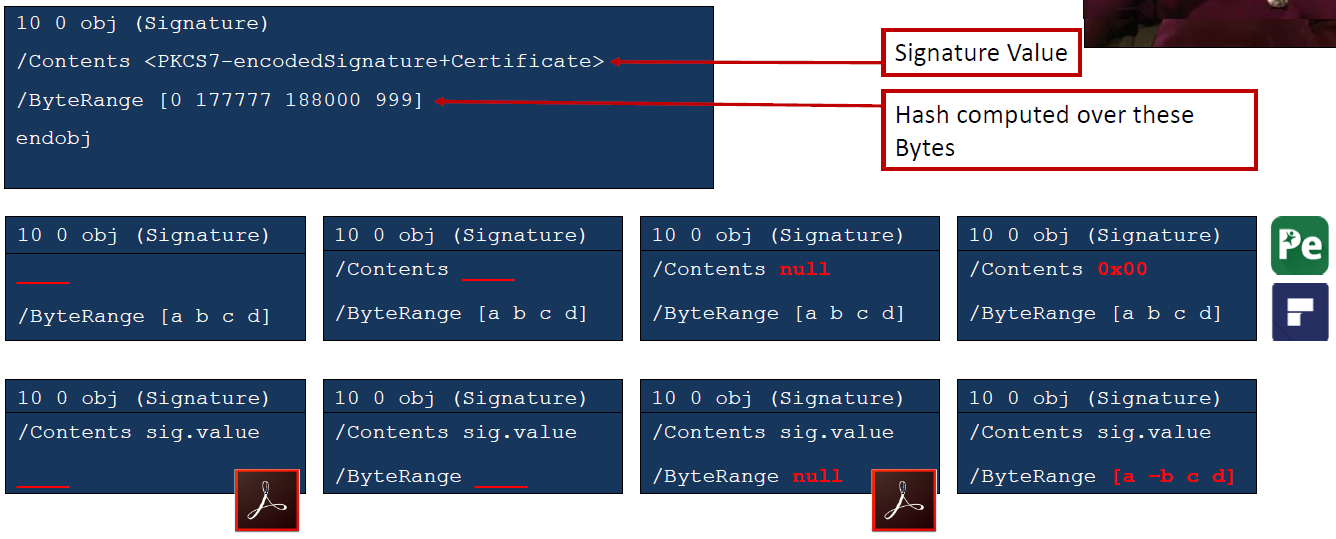
\includegraphics[width=0.8\textwidth]{"images/univ_sig_forgery.png"}
	\caption{\gls{usf}-Varianten \cite{ccc-break-pdf-slides}}
	\label{fig:usf}
\end{figure}

Mittels dieser Attacken ist es den Forschern gelungen zu zeigen, dass 21 von 22 PDF-Viewer inklusive denen von Adobe und 6 von 8 Online-Anbieter anfällig waren. Der einzige PDF-Viewer, der gegen alle Attacken immun war, war die veraltete Version von Adobe Reader 9, die jedoch remote code execution enthält \cite{ccc-break-pdf}. 
\subsection{PDFex PDF Encryption Attacks}
PDFex bezeichnet Attacken auf die PDF-Verschlüsselung mit Passwortschutz, die im Jahr 2019 entdeckt wurden. Die Forscher haben 27 PDF-Viewer auf diese Attacken getestet und alle Viewer inklusive Adobe Reader, Chrome and Firefox waren mindestens für eine Attacke anfällig. Es gibt 2 Attack-Klassifizierungen: Direct Exfiltration und \gls{cbc} Malleability Gadgets.
Das Attacker Model gestaltet sich wie folgt: 2 Personen Alice und Bob wollen ein vertrauliches PDF mit Passwort austauschen. Wir nehmen an, dass ein Angreifer durch eine \gls{mitm} Attack das verschlüsselte PDF unbemerkt abgreifen konnte als Alice das Dokument zu Bob geschickt hat. Daraufhin modifiziert der Angreifer das Dokument, sodass die Veränderungen unerkennbar sind für Bob, und schickt seine Version des Dokuments an Bob. Bob entsperrt das Dokument mit seinem Passwort und das entschlüsselte PDF wird automatisch zurück zum Server des Angreifers übertragen. \cite{ccc-break-pdf, pdfex}
\par
Ein verschlüsseltes PDF enthält einen Objekt-Stream als verschlüsselten Cipher Text im Body und einen /Encrypt-Eintrag, der Informationen darüber enthält, wie die Daten entschlüsselt werden sollen. Der Großteil der PDF-Dateistruktur liegt unverschlüsselt vor. Ausschließlich alle Strings und Streams für Inhalte ohne die anderen Objekttypen wie Integer oder Booleans, die dokumentstrukturbeschreibend sein sollen, werden verschlüsselt. Der Grund dafür ist, dass die PDF-Spezifikation weiterhin die random-access Optimierung im Dateiformat beibehalten möchte. Folglich ist die gesamte Dokumentenstruktur unverschlüsselt und eine ganze Reihe an wichtigen Informationen wie Anzahl und Größe der Seiten, verwendete Objekte oder Hyperlinks können vom Angreifer inspiziert werden. \\
PDF verwendet einen speziellen Streamfilter-Typ, genannt Crypt Filter für Verschlüsselung. Jeder Standard Filter eines Streams kann vom Crypt Filter überschrieben werden. Ein Standard Identity Filter wird bei besonderen Streams für z.B. Dokumentmetadaten gesetzt, damit diese unverschlüsselt bleiben in einem verschlüsselten Dokument. Diese Unterstützung von partieller Verschlüsselung kann einem Angreifer ermöglichen seinen Inhalt mit verschlüsseltem zu vermischen ohne das Passwort zu wissen. Forscher fanden 18 verschiedene Techniken für eine ganze Reihe von PDF-Readern. \cite{ccc-break-pdf}
\par
Bei der Direct Exfiltration Attack wird die Kryptografie nicht angerührt. Bei allen Strings im verschlüsselten PDF von Alice ändert der Angreifer die Crypt Filter zum Identity Filter um. Jetzt kann der Angreifer bei Bedarf Strings verändern und kann weitere Objekte mit unverschlüsselten Strings hinzufügen. Außerdem kann er verschlüsselte Teile des Dokuments in Inhalte einfügen, die er kontrolliert, d.h. er kann auf verschlüsselte Streams oder Strings in seinem Inhalt referenzieren und zugreifen. Nachfolgend fügt er eine submit-form action hinzu, die Namen und Werte von AcroForms zu einer Ziel-URL überträgt. Der Text des Formularfeldes wird als Stream gespeichert. Kombiniert der Angreifer eine OpenAction, die ausgeführt wird, sobald das Dokument geöffnet wird, mit einer submit-form action zu attacker.com, so kann der vertrauliche entschlüsselte Inhalt an den Angreifer zurück als POST-Request gesendet werden. Die OpenAction wird ausgelöst, sobald Bob sein Passwort eingegeben hat. Statt einer sumbit-form action kann man auch einen Hyperlink verwenden. Jedes Objekt kann als Hyperlink definiert werden, was einen Get-Request to attacker.com triggert. JavaScript kann ebenfalls verwendet werden. \cite{ccc-break-pdf, pdfex}
\par
PDF verschlüsselt durch \gls{aes}-256 mit einer Schlüssel-Länge von 256 Bit und operiert im \gls{cbc} Mode ohne \gls{mac} Integritätsschutz. \gls{aes} gehört zu den Blockchiffren und ist ein symmetrisches Verschlüsselungsverfahren. Bei symmetrischer Verschlüsselung gibt es nur einen Schlüssel fürs Verschlüsseln und Entschlüsseln. Ein Block ist 128 Bit lang. Der Subkey (Rundenschlüssel) hat immer eine Länge von 128 Bit. Die Schlüssellänge beeinflusst den key schedule, d.h. die Art und Weise wie Rundenschlüssel vom Master Key abgeleitet werden, sowie die Anzahl an Runden. Während der Algorithmus ausgeführt wird, wird ein 4 x 4 Array aus je 1 Byte (insgesamt 128 Bit), genannt State, in 14 Runden verschlüsselt. Im ersten einzigen Schritt, der KeyExpanion, werden die Rundenschlüssel für jede Runde plus 1 weiterer Rundenschlüssel aus dem Master Key berechnet. Anfangs wird der State gleichgesetzt mit dem der zu unverschlüsselten Nachricht (Plaintext). Auf dem State Array wird bitweises XOR mit dem Rundenschlüssel angewendet im AddRoundKey-Schritt. Jedes Byte vom State wird dabei mit einem Byte vom Rundenschlüssel kombiniert. Im SubBytes (Substitution) Schritt wird jedes Byte des aktualisierten State Arrays mit einem Byte durch eine Substitutionstabelle (S-Box) ersetzt. Dadurch werden die Bytes im State vermischt. Danach kommt die SchriftRows Sequenz. Die Bytes in jeder Zeile von State werden unterschiedlich nach links verschoben: Die 1. Zeile bleibt unberührt, die 2. Zeile wird um 1 verschoben, die 3. um 2 und die letzte um 3 Positionen. Die überlaufenden Zellen werden rechts an die jeweilige Zeile wieder angehängt. Als Vorletztes jeder Runde außer der letzten Runde kommt MixColumn dran. Hier werden Spalten vermischt, indem jede Spalte mit einer konstanten Matrix zu einer neuen Spalte multipliziert wird. Abschließend zu jeder Runde wird nochmals AddRoundKey mit dem aktuellen Rundenschlüssel ausgeführt, also State bitweise XOR verknüpft mit dem Rundenschlüssel. Im letzten Schritt produziert AddRoundKey den Ciphertext. Die invertierte Operation des Algorithmus wird beim entschlüsseln angewendet und alle Funktionen werden umgekehrt aufgerufen. \cite{intro-crypto, studyflix-aes, simply-aes} \\
Während des \gls{cbc} Mode wird ein vorheriger Ciphertextblock mit dem nächsten Plaintextblock durch XOR verknüpft. Das Ergebnis und der Schlüssel dienen als Input für den \gls{aes}-Algorithmus und produzieren einen verschlüsselten Output als Ciphertextblock. Im ersten Schritt wird der erste Plaintextblock mit einem Initialisierungsvektor IV (nonce) als Zufallszahl oder Zeitstempel mit XOR verknüpft. IV sollte nur einmal verwendet werden uns muss Sender und Empfänger bekannt sein. \cite{crypto-web} \\
Ein \gls{mac} ist eine kryptographische Prüfsumme, die aus dem Datensatz und dem symmetrischen Schlüssel von Sender und Empfänger gebildet wird. Im Gegensatz zu einem Hash kann der \gls{mac} nur von Sender und Empfänger berechnet und von beiden verifiziert werden. \cite{crypto-web}
\par
Nicht alle PDF-Viewer unterstützen teilweise verschlüsselte Dokumente. Sie sind immun gegen Direct Exfiltration Attacks. Trotzdem können Angreifer \gls{cbc} Malleability Gadgets verwenden, um die Exfiltrationen des Texts zu erhalten, da keine \gls{mac} für den Ciphertext beim PDF-Standard verwendet wird. Für die Ausführung der Attacke müssen 2 Vorbedingungen erfüllt sein. Zum einen muss ein Plaintext-Segment dem Angreifer vorliegen. Beim aktuellsten \gls{aes}V3-Algorithmus kann der Plaintext als 16 Bytes aus dem verschlüsselten /Perms Entry (extended permissions) einer PDF-Datei abgeleitet werden. Die zweiten 4 Bytes sind die permissions /P, die unverschlüsselt im PDF-Dokument herausgelesen werden können. Das Byte aus T oder F wird entsprechend des EncryptMetadate Booleans gesetzt. Der /Perms Entry wird mit dem gleichen Schlüssel für Streams und Strings verschlüsselt, daher kann man ihn verwendet um \gls{cbc} gadgets zu konstruieren. Obwohl der Perms-Wert mit \gls{ecb} Mode verschlüsselt wird, ist der Output-Ciphertext gleich seinem Plaintext, wenn man ihn mit \gls{cbc} verschlüsseln und dabei einen Initialization Vector von 0 verwendet würde. Bei älteren Versionen des \gls{aes}-Algorithmus in PDF muss der bekannte Plaintext aus dem Objekt, auf das die Exfiltration angewendet werden soll, extrahiert. \cite{ccc-break-pdf, pdfex} \\
Alice verschlüsselt eine Nachricht aus 2 Blöcken p0 und p1 zum Initialization Vector IV, c0 und c1 und Bob kann diese Nachricht wieder zu p0 und p1 entschlüsseln. \gls{cbc} Gadgets kann man konstruieren mit einem bekannten Plaintext-Teil p0, den man besitzt und kann dadurch neue Plaintextblöcke g0 und g1 in eine entschlüsselte Plaintext-Nachricht einfügen. Beispielsweise könnte g1 die URL vom Angreifer enthalten, sodass er sich die entschlüsselte Nachricht p1 von Alice an Bob auf seinen Server schicken lassen kann. Der Angreifer erhält die Nachricht aus IV, c0 und c1 von Alice durch eine \gls{mitm} Attacke und konstruiert 2 neue verschlüsselte Ciphertext Blöcke x0 und x1. Nimmt man IV XOR p0 erhält man einen Plaintext mit ausschließlich Nullen. X0 als vom Angreifer erstellter IV wird durch IV XOR p0 XOR g0 und x1 durch IV XOR p0 XOR g1 gebildet. Eine neue verschlüsselte Nachricht wird durch die Concatenation von x0, c0, x1, c0 und c1 gebildet. Der ursprüngliche c0 Block wird 2 Mal verwendet. X0 ist der neue IV und x1 ist lediglich dazu da, die Verkettung beizubehalten. X1 wird zu unkontrollierbaren Bytes ohne Sinn entschlüsselt. C1 ist der verschlüsselte Block von Alice, der die Zieldaten, enthält. Bei der Entschlüsselung erhält Bob den vom Angreifer erstellten Plaintext-Block g0, die unkontrollierten Bytes, den zweiten Plaintext-Block vom Angreifer g1 und die entschlüsselten Zieldaten von Alice. Folglich konnte der Angreifer Alices p0 durch g0 und g1 ersetzen. Als Exfiltration Channel kommen AcroForms oder Hyperlinks in Frage, um die entschlüsselte Nachricht von Bob zurück an den Angreifer zu schicken. \cite{gadget, pdf-insec-gadget, ccc-break-pdf}
\par
Hauptursache des Problems ist, dass viele Datenformate eine Teilverschlüsselung erlauben, z.B. \gls{xml}, S/\gls{mime} und PDF, was dem Angreifer ermöglicht eigene Inhalte einzuschleusen und Exfiltration Channels bilden kann. Des Weiteren \gls{aes}-\gls{cbc} enthält keinen Integritätsschutz wie einen \gls{mac}, sogar in PDF 2.0. Diese Sicherheitslücken sollten ohne Rückwärtskompatibilität in zukünftigen PDF-Spezifikationen entfernt werden. \cite{pdfex}
